%%%%%%%%%%%%%%%%%%%%%%%%%%%%%%%%%%%%%%%%%%%%%%%%%%%%%%%%%%%%%%%%%%%%%%%%%%%%%%%%%%%%%%%%%%%%%%%%%%%
\documentclass[10pt, a4paper]{article}
%%%%%%%%%%%%%%%%%%%%%%%%%%%%%%%%%%%%%%%%%%%%%%%%%%%%%%%%%%%%%%%%%%%%%%%%%%%%%%%%%%%%%%%%%%%%%%%%%%%

%--------------------------------------------------------------------------------------------------
% Dimensions :
%--------------------------------------------------------------------------------------------------

\setlength{\textheight}{26cm}
\setlength{\textwidth}{16cm}

\setlength{\topmargin}{-25mm}
\setlength{\oddsidemargin}{0mm}
\setlength{\evensidemargin}{0mm}

% \setlength{\columnsep}{20mm}

\setlength{\fboxsep}{1mm}
\setlength{\unitlength}{1mm}

%--------------------------------------------------------------------------------------------------
% Packages :
%--------------------------------------------------------------------------------------------------

\usepackage{latexsym}
\usepackage{graphicx}
\usepackage{pifont}
\usepackage{color}
\usepackage{amsmath}
\usepackage{amssymb}
\usepackage{enumerate}

\usepackage[french]{babel}    % pour franciser le document

%\usepackage[latin1]{inputenc} % pour utiliser les caracteres accentues du claviers
\usepackage[utf8]{inputenc} 

\usepackage{accents}

\usepackage{cancel}
% Style des vecteurs : fleche ou gras ?

%\newcommand{\myvec}[1]{\boldsymbol{#1}}
\newcommand{\myvec}[1]{\vec{#1}}

\newcommand{\mytensor}[1]{\accentset{\Rightarrow}{#1}} % needs \usepackage{accents}

%---------------------------
% Operateurs differentiels :
%---------------------------

\newcommand{\divergence}{\mbox{\rm div}\,}

\newcommand{\gradient}{\myvec{\mbox{\rm gra}}\mbox{\rm d}}
% \newcommand{\gradient}{\mathbf{grad}\,}
% \newcommand{\ggradient}{\stackrel{\Rightarrow}{\mbox{gra}}\!\!\!\,\mbox{d}\,}
\newcommand{\ggradient}{\accentset{\Rightarrow}{\mbox{\rm gra}}\mbox{\rm d}\!}

%\renewcommand{\dot}[1]{\accentset{\hbox{\huge .}}{#1}}
\newcommand{\mydot}[1]{\accentset{\centerdot}{#1}}

\newcommand{\rot}{\vec{\mbox{\rm ro}}\mbox{\rm t}\,}
%\newcommand{\rot}{\mathbf{rot}\,}

% \newcommand{\vnabla}{\vec{\nabla}}
\newcommand{\vnabla}{\boldsymbol{\nabla}}

% Fonctions speciales:

\newcommand{\besselj}[1]{\mbox{J}_{#1}}
\newcommand{\besselk}[1]{\mbox{K}_{#1}}
\newcommand{\bessely}[1]{\mbox{Y}_{#1}}
\newcommand{\besseli}[1]{\mbox{I}_{#1}}

% Vecteurs, tenseurs et torseurs:

\newcommand{\ex}{\mathbf{e}_{x}}
\newcommand{\ey}{\mathbf{e}_{y}}
\newcommand{\ez}{\mathbf{e}_{z}}

\newcommand{\er}{\mathbf{e}_{r}}
\newcommand{\erho}{\mathbf{e}_{\rho}}
\newcommand{\ephi}{\mathbf{e}_{\varphi}}
\newcommand{\etheta}{\mathbf{e}_{\theta}}

%\newcommand{\tensor}[1]{\stackrel{\Rightarrow}{#1}}
\newcommand{\tensor}[1]{\mbox{\sl \textbf{#1}}}
\newcommand{\torseur}[4]{
   \!\!\!\! \left . \begin{array}{c} \\ \\ _#1 \end{array} \!\!\!
   \right \{ \!\!\!
   \begin{array}{#4} #2 \\ \\ #3 \end{array}}

% Integrales multiples:

\newcommand{\odblint}[1]{\int\!\!\!\!\!\int_{#1} \hskip -7mm \bigcirc \;}
\newcommand{\dblint}{\int\!\!\!\!\!\int}
\newcommand{\tplint}{\int\!\!\!\!\!\int\!\!\!\!\!\int}

% Fractions:

\renewcommand{\dfrac}[2]{\displaystyle \frac{#1}{#2}}

% Derivees ordinaires et partielles:

\newcommand{\dpdt}[1]{\dfrac{\partial #1}{\partial t}}
\newcommand{\dpdx}[1]{\dfrac{\partial #1}{\partial x}}
\newcommand{\dpdy}[1]{\dfrac{\partial #1}{\partial y}}
\newcommand{\dpdz}[1]{\dfrac{\partial #1}{\partial z}}

\newcommand{\ddpdt}[1]{\dfrac{\partial^2 #1}{\partial t^2}}
\newcommand{\ddpdx}[1]{\dfrac{\partial^2 #1}{\partial x^2}}
\newcommand{\ddpdy}[1]{\dfrac{\partial^2 #1}{\partial y^2}}
\newcommand{\ddpdz}[1]{\dfrac{\partial^2 #1}{\partial z^2}}

\newcommand{\dpdr}[1]{\dfrac{\partial #1}{\partial r}}
\newcommand{\dpdrho}[1]{\dfrac{\partial #1}{\partial \rho}}
\newcommand{\dpdphi}[1]{\dfrac{\partial #1}{\partial \varphi}}
\newcommand{\dpdtheta}[1]{\dfrac{\partial #1}{\partial \theta}}

\newcommand{\ddpdr}[1]{\dfrac{\partial^2 #1}{\partial r^2}}
\newcommand{\ddpdrho}[1]{\dfrac{\partial^2 #1}{\partial \rho^2}}
\newcommand{\ddpdphi}[1]{\dfrac{\partial^2 #1}{\partial \varphi^2}}
\newcommand{\ddpdtheta}[1]{\dfrac{\partial ^2#1}{\partial \theta^2}}

\newcommand{\ddt}[1]{\dfrac{d #1}{dt}}
\newcommand{\ddx}[1]{\dfrac{d #1}{dx}}
\newcommand{\ddy}[1]{\dfrac{d #1}{dy}}
\newcommand{\ddz}[1]{\dfrac{d #1}{dz}}
\newcommand{\ddr}[1]{\dfrac{d #1}{dr}}

\newcommand{\ddtref}[2]{\dfrac{d #1}{dt}_{\! | #2 }}
\newcommand{\dpdtref}[3]{\dfrac{\partial #1}{\partial #2}_{\! | #3 }}

% Misc:

\newcommand{\mycaption}[1]{\caption{\sl #1}}

\newcommand{\ligne}[1]{\hrule height #1\linethickness \hfill}

\newcommand{\thickline}[2]{\linethickness{#1} \line(1, 0){#2}}

\newcommand{\myline}{\noindent\underline{\hspace{\textwidth}}}
\newcommand{\mysection}[1]{\vskip 0.5cm \section{#1}\vskip -1.4cm 
   \myline \vskip 0.4cm \myline \bigskip}

\newcommand{\etal}{\textit{et al.}}

\newcommand{\varray}[1]{\renewcommand{\arraystretch}{#1}}

\newcommand{\puissance}[1]{^{\mbox{\footnotesize #1}}}
\newcommand{\indice}[1]{_{\mbox{\footnotesize #1}}}

%---------------------------------------------------------------------
% New environments:
%---------------------------------------------------------------------

\newcounter{MyEnumCounter}
\newcounter{MySaveCounter}
\newenvironment{MyEnum}{%
  \begin{list}{\arabic{MyEnumCounter}.}{\usecounter{MyEnumCounter}%
  \setcounter{MyEnumCounter}{\value{MySaveCounter}}}
  }{%
  \setcounter{MySaveCounter}{\value{MyEnumCounter}}\end{list}%
}
\newcommand{\MyEnumReset}{\setcounter{MySaveCounter}{0}}

\newenvironment{deuxcols}{\begin{tabular}{lr} \hspace*{-9.7mm}}{\end{tabular}}

\newenvironment{dem}{\noindent %
   \begin{tabular}{||l} \textsl{D\'emonstration :} \\ % 
   \begin{minipage}{15.5cm} \footnotesize} %
   {\end{minipage}\end{tabular}}

\newenvironment{abst}{\begin{quotation}\sl}{\end{quotation}}

\newenvironment{eqnbox}{\begin{equation}\begin{array}{|c|}  \hline \\ 
   \displaystyle}{\\ \\ \hline \end{array} \end{equation}}

\newcommand{\myprime}{\ \!'}

% JFM symbols:

\DeclareMathSymbol{\varGamma}{\mathord}{letters}{"00}
\DeclareMathSymbol{\varDelta}{\mathord}{letters}{"01}
\DeclareMathSymbol{\varTheta}{\mathord}{letters}{"02}
\DeclareMathSymbol{\varLambda}{\mathord}{letters}{"03}
\DeclareMathSymbol{\varXi}{\mathord}{letters}{"04}
\DeclareMathSymbol{\varPi}{\mathord}{letters}{"05}
\DeclareMathSymbol{\varSigma}{\mathord}{letters}{"06}
\DeclareMathSymbol{\varUpsilon}{\mathord}{letters}{"07}
\DeclareMathSymbol{\varPhi}{\mathord}{letters}{"08}
\DeclareMathSymbol{\varPsi}{\mathord}{letters}{"09}
\DeclareMathSymbol{\varOmega}{\mathord}{letters}{"0A}

% ---------------------------------------------------------------------
% MISC SYMBOLS :
% ---------------------------------------------------------------------

\font\SY=msam10 
\def\carreblanc{\hbox{\SY \char'3}}
\def\carrenoir{\hbox{\SY \char'4}}
\def\diamblanc{\hbox{\SY \char'6}}
\def\diamnoir{\hbox{\SY \char'7}}
\def\triblancright{\hbox{\SY \char'102}}
\def\triblancleft{\hbox{\SY \char'103}}
\def\triblancup{\hbox{\SY \char'115}}
\def\triblancdown{\hbox{\SY \char'117}}
\def\trinoirright{\hbox{\SY \char'111}}
\def\trinoirleft{\hbox{\SY \char'112}}
\def\trinoirup{\hbox{\SY \char'116}}
\def\trinoirdown{\hbox{\SY \char'110}}
\def\rondblanc{\hbox{\scriptsize $\bigcirc$}}
\def\rondnoir{\hbox{\LARGE $\bullet$}}

\font\BB=msbm10 scaled 1095
\def\setr{\hbox{\BB R}}
\def\setc{\hbox{\BB C}}
\def\setn{\hbox{\BB N}}
\def\setz{\hbox{\BB Z}}

% Pour enlever la numerotation des pages de la table des matieres:

%%%% debut macro, a placer dans preambule %%%%
\makeatletter
\def\addcontentsline@toc#1#2#3{%
   \addtocontents{#1}{\protect\thispagestyle{empty}}%
   \addtocontents{#1}{\protect\contentsline{#2}{#3}{\thepage}}}
\def\addcontentsline#1#2#3{%
  \expandafter\@ifundefined{addcontentsline@#1}%
  {\addtocontents{#1}{\protect\contentsline{#2}{#3}{\thepage}}}
  {\csname addcontentsline@#1\endcsname{#1}{#2}{#3}}}
\makeatother
%%%% fin macro %%%%

\newcommand{\titre}[1]{ %
  \medskip \noindent \underline{\makebox[\textwidth][l]{\textbf{#1}\textcolor{white}{pl}}}}% \\}

\newcommand{\sstitre}[1]{ %
  \bigskip \centerline{\textbf{#1}} \smallskip}

\def\draft{\overfullrule 5pt} % The \draft command marks the overful boxes

\def\indentlist{\list%
        {}{\labelwidth 0pt \leftmargin 3\labelsep}}
\let\endindentlist\endlist \relax

\def\datelist{\list%
        {}{\settowidth\labelwidth{[2001/02 :]}
        \leftmargin\labelwidth
        \advance\leftmargin\labelsep}
}
\let\enddatelist\endlist \relax

\def\longuelist{\list%
        {}{\settowidth\labelwidth{[Etablissement :]}
        \leftmargin\labelwidth
        \advance\leftmargin\labelsep}
}
\let\endlonguelist\endlist \relax

\def\shortlist{\list%
        {}{\settowidth\labelwidth{$\bullet$}
        \leftmargin\labelwidth
        \advance\leftmargin\labelsep}
}
\let\endshortlist\endlist \relax



%--------------------------------------------------------------------------------------------------
% Divers :
%--------------------------------------------------------------------------------------------------

\definecolor{rougefonce}{rgb}{0.7, 0.2, 0.2}

\renewcommand{\thickline}[2]{\linethickness{#1} \line(1, 0){#2}}
\renewcommand{\mycaption}[1]{\caption{\sl #1}}
\renewcommand{\myvec}[1]{\vec{#1}}

\newcommand{\footnoteremember}[2]{
\footnote{#2}
\newcounter{#1}
\setcounter{#1}{\value{footnote}}% \!\!\!
}
\newcommand{\footnoterecall}[1]{
\footnotemark[\value{#1}]
}

% \pagestyle{empty}

\graphicspath{{../FIGURES/}{Figures/}} % chemin d'acces au repertoire des figures (par ex.)

%%%%%%%%%%%%%%%%%%%%%%%%%%%%%%%%%%%%%%%%%%%%%%%%%%%%%%%%%%%%%%%%%%%%%%%%%%%%%%%%%%%%%%%%%%%%%%%%%%%
\begin{document}
%%%%%%%%%%%%%%%%%%%%%%%%%%%%%%%%%%%%%%%%%%%%%%%%%%%%%%%%%%%%%%%%%%%%%%%%%%%%%%%%%%%%%%%%%%%%%%%%%%%

\begin{center}

  \textsc{Université Toulouse 3 -- Paul Sabatier \hfill Année universitaire 2017-2018}
  
  \textsc{Mécanique des fluides \hfill L3 Mécanique}
  
  \vspace{0mm}
  
  \begin{center}
    \thickline{0.4mm}{160}
    \\ \vspace{3mm}
  \textbf{\large Exercice complémentaire 4 : écoulement de Poiseuille}
    \\ %\vspace{1mm}
    \thickline{0.4mm}{160}
  \end{center}

  %\vspace{5mm}
  
\end{center}

\bigskip
On considère l'écoulement incompressible d'un fluide newtonien homogène 
de masse volumique $\rho$ dans une conduite de section circulaire de rayon $R$ 
et de grande longueur $L$ suivant l'axe $Oz$ (fig.~\ref{fig:conduite}).
Le fluide dans la conduite est mis en écoulement sous l'action d'une différence 
de pression entre l'entrée et la sortie de la conduite.
Sans perte de généralité on supposera $P_1>P_2$, et on notera $G = (P_1-P_2)/L$ le gradient de pression entre l'entrée et la sortie.
On négligera les forces massiques (dont la pesanteur).
On notera $\nu$ et $\mu = \rho \nu$ les viscosités cinématique et dynamique.
La géométrie du problème conduit naturellement à travailler dans un repérage cylindrique $(r, \theta, z)$.

\begin{figure}[hbt]
  \begin{center}
    \begin{picture}(150, 20)(0, 5)
      \put(0, 0){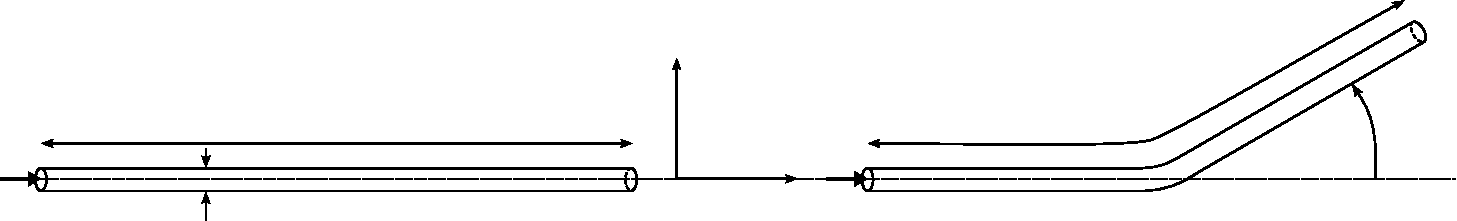
\includegraphics[width=145mm]{conduite.pdf}}
      \put(147, 11){ $z$}
      \put(42, 15){ $R$}
      \put(76, 14){ $r$}
      \put(97, 14){ $u(r)$}
      \put(58, 24){ $dz$}
      \put(64, 0.7){\colorbox{white}{$L\gg R$}}
      \put(1, 13){$P_1$}
      \put(137, 13){$P_2$}
    \end{picture}
  \end{center}
  \mycaption{Ecoulement laminaire en conduite cylindrique.}
  \label{fig:conduite}
\end{figure}

%==================================================================================================
\section{Recherche d'une solution particulière}
%==================================================================================================

Les équations de la mécanique des fluides étant non linéaires, 
il existe potentiellement plusieurs solutions d'écoulements 
pour une même configuration géométrique et opérationnelle (mêmes conditions limites).
La plupart de ces solutions ne sont pas accessibles par le calcul analytique et sont même difficiles
à calculer numériquement sur ordinateur.
En particulier les solutions instationnaires et tridimensionnelles d'écoulements en conduite restent
un sujet actuel d'étude pour les ingénieurs et les chercheurs.

Dans ce contexte, l'objectif ici n'est pas de trouver toutes les solutions d'écoulements, 
mais de déterminer parmi celles-ci la solution la plus simple qui, tout en respectant bien sûr
les conditions physiques du problème (c'est une "vraie" solution \textsl{exacte} du problème) 
permet une résolution analytique.

\begin{enumerate}
\item 
Justifier en quelques mots pourquoi il est légitime de rechercher a priori une solution :
\begin{enumerate}[a)]
\item 
  ne dépendant pas du temps
  (écoulement \textsl{permanent} ou \textsl{stationnaire}) $\myvec{u} = \myvec{u}(r, \theta, z)$,
\item 
	ne dépendant pas de $z$
	(écoulement \textsl{établi}) $\myvec{u} = \myvec{u}(r, \theta)$,
\item
	ni de $\theta$ (écoulement \textsl{axisymétrique}) $\myvec{u} = \myvec{u}(r)$,
\item 
	et correspondant à un écoulement purement axial (écoulement \textsl{unidirectionnel}\,)
	\begin{equation}
		\myvec{u} = u(r) \, \ez
		\label{eq:solution}
	\end{equation}
\end{enumerate}
\item
	Vérifier que ce type de solution correspond bien à un écoulement 
	incompressible\footnoteremember{cylindriques}{
	Les expressions de l'équation de Navier-Stokes incompressible 
	et du tenseur des contraintes en repérage cylindrique 
	sont disponibles en annexe du fascicule de TD.}\!\!.
\item
	Exprimer le tenseur des contraintes\footnoterecall{cylindriques} \!\!\!
	$\mytensor{\sigma}$ pour cette solution d'écoulement particulière.
\end{enumerate}

%==================================================================================================
\section{Mise en équation}
%==================================================================================================

Il s'agit dans cette partie de mettre en équation l'écoulement en conduite
dans le cadre des données et des hypothèses du problème.

\begin{enumerate}
\item
Une première méthode consiste simplement à injecter dans l'équation de Navier-Stokes 
incompressible\footnoterecall{cylindriques}
le type de solution particulière (\ref{eq:solution}) identifiée dans la section précédente.
\begin{enumerate}[a)]
\item 
Montrer que la pression ne dépend ni de $r$ ni de $\theta$ : $p=p(z)$.
\item
Montrer que le gradient de pression $dp/dz$ est constant le long de la conduite et donner sa valeur en fonction des données du problème.
\item
En déduire que l'équation à résoudre pour le champ de vitesse est
\begin{equation}
	\dpdr{} \left ( r \dpdr{u}\right ) = -\frac{Gr}{\mu}
\label{eq:equation}
\end{equation}
\end{enumerate}
\item
Question subsidiaire : 
une autre méthode consiste à dériver l'équation pour $u$ à partir d'un bilan de quantité de mouvement.
Il n'est en effet pas nécessaire d'avoir écrit les équations de Navier-Stokes dans le cas général pour l'appliquer dans ce cas particulier : il suffit de remonter au bilan de quantité de mouvement sur un volume de contrôle
élémentaire et de l'écrire dans le cas particulier (\ref{eq:solution}).
\begin{enumerate}[a)]
\item 
	Au préalable, justifier en quelques mots pourquoi la pression ne dépend que de $z$ a priori.
\item
	En écrivant le bilan de quantité de mouvement \textsl{suivant $z$} pour le volume de contrôle
	de rayon $r$ et de longueur infinitésimale $dz$ (fig.~\ref{fig:conduite}),
	montrer que 
	\[
		\tau(r) = -\dfrac{Gr}{2}
	\]
	où $\tau(r) = \tau_{rz}(r)$ désigne la composante $rz$ du tenseur des contraintes visqueuses.
\item
	Dans l'hypothèse d'un fluide newtonien, en déduire l'équation différentielle
	à satisfaire pour $u$.
\end{enumerate}
\end{enumerate}

%==================================================================================================
\section{Résolution et applications}
%==================================================================================================

La résolution de l'équation (\ref{eq:equation}) issue de la modélisation requiert la prise en compte
des conditions aux limites.
On supposera que la paroi de la conduite est fixe et imperméable, et qu'il y a \textsl{adhérence}
à la paroi. Par conséquent $\myvec{u} = \myvec{0}$ en $r=R$.
D'autre part, la réalité physique interdit d'avoir des vitesses infinies, et on supposera 
donc que la vitesse sur l'axe $r=0$ est finie.

\begin{enumerate}
\item
	Dans ces conditions, déterminer la vitesse $u(r)$ et tracer le profil de vitesse associé.
	L'écoulement correspondant à cette solution\footnote{Voir 
	l'article sur Wikipedia : \texttt{fr.wikipedia.org/wiki/Ecoulement\_de\_Poiseuille}}
  est appelé \textsl{écoulement de Poiseuille}.
	Cette solution d'écoulement est effectivement observée dans les conduites pour des nombres
	de Reynolds $Re=UD/\nu$ inférieurs à 2000 environ ($D=2R$ désigne le diamètre de la conduite). 
\item
	Calculer le débit massique $\dot{m}$ passant dans la conduite
	puis en déduire le débit volumique $q$ et la vitesse moyenne $U$,
	aussi appelée \textsl{vitesse débitante}.
	Comparer à la vitesse maximale $U\indice{max}$.
\item[]
	Remarque :
	l'expression du débit volumique en fonction du gradient de pression 
	trouvée précé\-demment constitue la \textsl{loi de Poiseuille} ou de \textsl{Hagen-Poiseuille}.
	Cette "loi" a été établie par
	Jean-Louis Marie Poiseuille, médecin et physicien français qui s'intéressait notamment 
	à la circulation du sang dans les vaisseaux.
	Une particularité réside dans la loi d'échelle du débit en fonction du rayon $R$ :
	le débit est en effet proportionnel au rayon à la puissance 4, 
	ce qui conduit à une dépendance très forte du débit
	vis-à-vis du rayon de la conduite, comme cela sera illustré en TD.
	Ainsi une conduite soumise à un gradient de pression donné, pour un fluide de viscosité donnée,
	dont le rayon est multiplié par 2 voit son débit multiplié par $2^4 = 16$ !
\item[]
	\textbf{Questions subsidiaires :}
\item
	Déterminer l'expression de la contrainte visqueuse $\tau(r)$ et discuter de son signe.
	Où l'intensité de cette contrainte est-elle maximale ? 
\item
	En déduire la force exercée par l'écoulement sur la conduite de longueur $L$.
%\item
%	Retrouver le résultat en écrivant un bilan global d'énergie cinétique dans la conduite.
\item
	Déterminer la dissipation d'énergie cinétique dans la conduite de longueur $L$.
\item
	La chute de pression dans la conduite correspond à une diminution de l'énergie mécanique 
	du fluide à cause des frottements visqueux. On parle alors de perte de charge régulière
	et on définit le coefficient de perte de charge par 
	\begin{equation}
		\lambda = \dfrac{D}{L} \times \dfrac{P_1-P_2}{\frac{1}{2} \rho U^2}
	\end{equation}	
	Vérifier que ce coefficient est sans dimension, et déterminer son expression en fonction
	du nombre de Reynolds dans le cas de l'écoulement de Poiseuille. 
\end{enumerate}

\medskip
\noindent
\textbf{Références :}

\medskip
Poiseuille J.-M. L. (1844) Le mouvement des liquides dans les tubes de petits diamètres.

%%%%%%%%%%%%%%%%%%%%%%%%%%%%%%%%%%%%%%%%%%%%%%%%%%%%%%%%%%%%%%%%%%%%%%%%%%%%%%%%%%%%%%%%%%%%%%%%%%%
\end{document}
%%%%%%%%%%%%%%%%%%%%%%%%%%%%%%%%%%%%%%%%%%%%%%%%%%%%%%%%%%%%%%%%%%%%%%%%%%%%%%%%%%%%%%%%%%%%%%%%%%%

